\documentclass[]{beamer}

\usetheme[block=fill]{metropolis}

\usepackage{graphicx} % Allows including images
\usepackage{amsmath,amsfonts,amsthm,amssymb}
\usepackage{color}
\usepackage{xcolor,cancel}
\usepackage{enumitem}
\setitemize{label=\usebeamerfont*{itemize item}%
	\usebeamercolor[fg]{itemize item}
	\usebeamertemplate{itemize item}}
\definecolor{mDarkBrown}{HTML}{604c38}
\definecolor{mDarkTeal}{HTML}{23373b}
\definecolor{mLightBrown}{HTML}{EB811B}
\definecolor{mMediumBrown}{HTML}{C87A2F}
\definecolor{mygreen}{HTML}{98C2B9}
\definecolor{myyellow}{HTML}{DFD79C}
\definecolor{myblue}{HTML}{8CA7CC}
\definecolor{kern}{HTML}{8CC2B7}


\usepackage{float}
\usepackage{framed}
\usepackage{epsfig}
\usepackage{graphicx}
\usepackage{subcaption}
\usepackage{ulem}
\usepackage{hhline}
\usepackage{multirow}
\usepackage{comment}   
\usepackage{bbm}
\usepackage{tikz}   
\def\Put(#1,#2)#3{\leavevmode\makebox(0,0){\put(#1,#2){#3}}}
\newcommand*\mystrut[1]{\vrule width0pt height0pt depth#1\relax}
\newcommand{\eqdef}{\mathbin{\stackrel{\rm def}{=}}}


\newcommand{\bs}[1]{\boldsymbol{#1}}
\newcommand{\bv}[1]{\mathbf{#1}}
\newcommand{\R}{\mathbb{R}}
\newcommand{\E}{\mathbb{E}}

\DeclareMathOperator*{\argmin}{arg\,min}
\DeclareMathOperator*{\argmax}{arg\,max}
\DeclareMathOperator{\nnz}{nnz}
\DeclareMathOperator{\Var}{Var}
\DeclareMathOperator{\sinc}{sinc}
\DeclareMathOperator{\mv}{mv}
\DeclareMathOperator{\sgn}{sgn}
\DeclareMathOperator{\step}{step}
\DeclareMathOperator{\gap}{gap}
\DeclareMathOperator{\poly}{poly}
\DeclareMathOperator{\tr}{tr}
\DeclareMathOperator{\orth}{orth}
\newcommand{\norm}[1]{\|#1\|}
\captionsetup[subfigure]{labelformat=empty}
\captionsetup[figure]{labelformat=empty}
\DeclareMathOperator*{\lmin}{\lambda_{min}}
\DeclareMathOperator*{\lmax}{\lambda_{max}}

\newcommand{\specialcell}[2][c]{%
	\begin{tabular}[#1]{@{}c@{}}#2\end{tabular}}
\newcommand{\specialcellleft}[2][c]{%
	\begin{tabular}[#1]{@{}l@{}}#2\end{tabular}
}

\usepackage{tabstackengine}
\stackMath


%----------------------------------------------------------------------------------------
%	TITLE PAGE
%----------------------------------------------------------------------------------------

\title{CS-GY 6763/CS-UY 3943: Lecture 1 \\ Course introduction, concentration of random variable, applications}
\author{NYU Tandon School of Engineering, Prof. Christopher Musco}
\date{}

\begin{document}
	
	\begin{frame}
		\titlepage 
	\end{frame}
	
	\metroset{titleformat=smallcaps}
	
	\begin{frame}
		\frametitle{algorithms in the age of data science}	
		\begin{center}
			\large\textbf{Algorithmic Machine Learning and Data Science}
			
			Statistics, machine learning, and data science study how to use data to make better decisions or discoveries.
			
			\vspace{1em}
			In this class, we study how to do so \alert{\textbf{as quickly as possible, or with limited computational resources.}}
			
			
		\end{center}
	\end{frame}
	
	\begin{frame}
		\frametitle{applications by the numbers}
		\begin{itemize}
			\item \textbf{X (Twitter)} receives 6,000 tweets \emph{every second}.
			\item \textbf{Google} receives $\approx$ 20,000 Maps queries \emph{every second}.
			\item \textbf{NASA} collects 6.4 TB of satallite images \emph{every day}. 
			\item \textbf{Rubin Observatory in Chile} will collect 20 TB of images \emph{every night}. 
			\item \textbf{MIT/Harvard Broad Institute} sequences 24 TB of genetic data \emph{every day}. 
		\end{itemize}
	\end{frame}
	
	\begin{frame}
		\frametitle{role of algorithms}
		\textbf{Growing demands of data science and machine learning have ushered in a new ``golden age'' for algorithms research.}
		\begin{itemize}
			\item Bolstered by our limited ability to build faster computers (or to access computational resources with a limited financial  budget). 
			\item Typical data applications require combining a diverse set of algorithmic tools. Most are not heavily covered in your traditional algorithms curriculum.
		\end{itemize} 
	\end{frame}
	
	\begin{frame}
		\frametitle{class topics}
		\begin{center}
			\begin{enumerate}[label=(\arabic*)]
				\item Randomized methods.
				\item Optimization.
				\item Spectral methods and linear algebra.
				\item Touch on Fourier methods.
			\end{enumerate}
			
			\vspace{1em}
			Focus is on teaching \emph{tools} to design algorithms, not just the algorithms themselves. 
		\end{center}
	\end{frame}
	
	\begin{frame}
		\frametitle{randomized methods}
		\small
		\textbf{Section 1: Randomized Algorithms.}
		
		\alert{\textbf{It is hard to find an algorithms paper in 2023 that does not use randomness in some way, but this wasn't always the case!}}
		\begin{itemize}
			\item Probability tools and concentration of random variables (Markovs, Chebyshev, Chernoff/Bernstein inequalities).
			\item Random hashing for fast data search, load balancing, and more. Locality sensitive hashing, MinHash, SimHash, etc.
			\item Sketching and streaming algorithms for compressing and processing data on the fly.
			\item High-dimensional geometry and the Johnson-Lindenstrauss lemma for compressing high dimensional vectors.
		\end{itemize}
	\end{frame}
	
	\begin{frame}
		\frametitle{continuous optimization}
		\small
		\textbf{Section 2: Optimization.}
		
		\alert{\textbf{Optimization has become the algorithmic workhorse of modern machine learning.}}
		\begin{itemize}
			\item Gradient descent, stochastic gradient descent, coordinate descent, and how to analyze these methods.
			\item Acceleration, conditioning, preconditioning, adaptive gradient methods.
			\item Constrained optimization, linear programming. Ellipsoid and interior point methods.
			\item Discrete optimization, relaxation, submodularity and greedy methods.
		\end{itemize}
	\end{frame}
	
	\begin{frame}
		\frametitle{spectral methods}
		\small
		
		\textbf{Section 3: Spectral methods and linear algebra.}
		
		\alert{\textbf{``Complex math operations (machine learning, clustering, trend detection) [are] mostly specified as linear algebra on array data'' -- Michael Stonebraker, Turing Award Winner}}
		
		\begin{itemize}
			\item How to compute singular value decompositions and eigendecomposition.
			\item Spectral graph theory: i.e. how to use linear algebara to understanding large graphs through linear algebra (social networks, interaction graphs, etc.). 
			\item Spectral clustering and non-linear dimensionality reduction.
			\item Random sampling and sketching methods for matrix computations.
		\end{itemize}
	\end{frame}
	
	\begin{frame}
		\frametitle{fourier methods}
		\small
		\textbf{Section 4: Fourier methods.}
		\begin{itemize}
			\item Compressed sensing, sparse recovery, and their applications.
			\item Fast Fourier Transform inspired methods in linear algebra and dimensionality reduction.
			\item Fourier perspective on machine learning techniques like kernel methods, and the algorithmic benefits.
		\end{itemize}
	\end{frame}
	
	\begin{frame}
		\frametitle{what we won't cover}
		
		\textbf{Software tools or frameworks.} Spark, Tensorflow, etc.  If you are interested, CS-GY 6513 might be a good course.
		\vspace{1em}
		
		\textbf{Machine Learning Models + Techniques.} Neural nets, reinforcement learning, Bayesian methods, unsupervised learning, etc. I assume you have already had a course in ML and the focus of this class is on \emph{computational considerations}.
		
		\begin{center}
			But if your research is in machine learning, I think you will find the theoretical tools we learn are more broadly applicable than in designing faster algorithms. 
		\end{center}
		
	\end{frame}
	
	
	\begin{frame}
		\frametitle{our approach}
		\small
		\begin{center}
			\alert{This is primarily a \textbf{theory} course.}
		\end{center}
		\begin{itemize}
			\item Emphasis on proofs of correctness, bounding asymptotic runtimes, convergence analysis, etc. \textit{Why?}
			\item Learn how to model complex problems in simple ways. 
			\item Learn general mathematical tools that can be applied in a wide variety of problems (in your research, in industry, etc.)
			\item The homework requires \textbf{creative problem solving} and thinking beyond what was covered in class. You will not be able to solve many problems on your first try!
		\end{itemize}
		You will need a good background in \textbf{probability} and \textbf{linear algebra}. See the syllabus for more details. Ask me is you are still unsure.
	\end{frame}
	
	
	%\begin{frame}
	%	\frametitle{target applications}
	%	\begin{itemize}
		%		\item \textbf{High thoughput and realtime data applications.}
		%		\begin{itemize}
			%			\item Google Maps/Waze
			%			\item Product recommendations, content recommendations
			%		\end{itemize}
		%		\item \textbf{High complexity machine learning models that require lots of training data}
		%		\begin{itemize}
			%		\item Deep neural networks
			%		\item Machine translation
			%		\end{itemize}
		%		\item \textbf{Data analysis on low-compute devices}
		%		\begin{itemize}
			%			\item Smartphones/watches
			%			\item Robots, drones
			%		\end{itemize}
		%	\end{itemize}
	%\end{frame}
	
	\begin{frame}
		\frametitle{course structure and logistics}
		\begin{center}
			All of this information is on the course webpage \url{https://www.chrismusco.com/amlds2023/} and in the syllabus posted there! Please take a look.
		\end{center}
		
		\textbf{Class structure:}
		\begin{itemize}
			\item Lecture once a week. You \emph{can} attend on Zoom, but I recommend coming in person.
			\item Office hours from me and TAs once a week.
		\end{itemize}
		
		\textbf{Tech tools:}
		\begin{itemize}
			\item \textbf{Website} for up-to-date info, lecture notes, readings.
			\item \textbf{Ed Discussion} for questions about material. 
			\item \textbf{Gradescope} for turning in assignments. Sign up using course code.
		\end{itemize}
		
		\begin{center}
		\end{center}
	\end{frame}
	
	
	
	\begin{frame}
		\frametitle{course structure and logistics}
		\textbf{Class work:}
		\begin{itemize}
			\item \textbf{5 problem sets} (50\% of course grade). 
			\begin{itemize}
				\item These are challenging, and the most effective way to learn the material. I recommend you start early, work with others, ask questions on Ed, etc.
				\item You must \emph{write-up} solutions on your own.\footnote{10\% bonus on first problem set for using Markdown or LaTex. It should save you time in the long run!} 
			\end{itemize}
			\item \textbf{Midterm (Oct. 20th)} {20}\% of course grade). 
		\end{itemize}
	\end{frame}
	
	\begin{frame}
		\frametitle{course structure and logistics}
		\textbf{Final project \emph{or} final exam (20\% of grade):}
		\begin{itemize}
			\item Final exam will be similar to midterm and problem sets. 
			\item Final project can be based on a recent algorithms paper, and can be either an experimental or theoretical project. \emph{Must work in a pair.}
			\item We will hold a \textbf{reading group} outside of class for those who decide to complete a final project to workshop topics and papers. 
			\item Others can join as well -- it's a great opportunity to get better at reading and presenting papers.
		\end{itemize}
	\end{frame}
	
	\begin{frame}
		\frametitle{course structure and logistics}
		\textbf{Class participation (10\% of grade):}
		\begin{itemize}
			\item My goal is to know you all individually by the end of this course.
			\item Lots of ways to earn the full grade: participation in lecture, office hours, or Ed discussion. Participation in the reading group. Effort on the project. 
		\end{itemize}
		\textbf{Important note:}
	\begin{itemize}
		\item This is a mixed undergraduate/graduate course. 
		\item Workload is the same, but undergraduates are graded on a different ``curve''.
	\end{itemize}
	\end{frame}
	
	\begin{frame}
		\frametitle{rockstar course team}
		\begin{center}
			\includegraphics[width=\textwidth]{courseTeam.png}
		\end{center}
	\textbf{Things to look forward to:}
	\begin{itemize}
		\item Teal's typeset lecture notes.
		\item Apoorv and Raphael's ``proof writing sessions''.
		\item Feyza's guest lecture on ``fine grained complexity''.
	\end{itemize}
	\end{frame}
	
	\begin{frame}[standout]
		\begin{center}
			questions?
		\end{center}
	\end{frame}
	
	\begin{frame}
		\frametitle{this class}
		\textbf{Goal:} Demonstrate how even the \emph{simplest tools} from probability can lead to a powerful algorithmic results. 
		
		\textbf{Lecture applications:}
		\begin{itemize}
			\item Estimating set size from samples. 
			\item Finding frequent items with small space.
		\end{itemize}
		\textbf{Problem set applications:}
		\begin{itemize}
			\item Group testing for COVID-19.
			\item Smarter load balancing. 
		\end{itemize}	
	\end{frame}
	
	\begin{frame}
		\frametitle{probability review}
		Let ${X}$ be a random variable taking value in some set $\mathcal{S}$. I.e. for a dice, $\mathcal{S} = \{1,\ldots, 6\}$. For a continuous r.v., we might have $\mathcal{S} = \R$.
		
		\begin{itemize}
			\item \textbf{Expectation}: \hspace{1em}$\E[X] = \sum_{s\in \mathcal{S}} \Pr[{X} = s]\cdot s$
			
			\vspace{.5em}
			For continuous r.v., $\E[X] = \int_{s\in \mathcal{S}} \Pr(s)\cdot s \,ds$.
			
			\vspace{1em}
			\item \textbf{Variance}: \hspace{1.2em} $\Var[X] = \E[(X - \E[X])^2]$
		\end{itemize}
		\begin{center}
			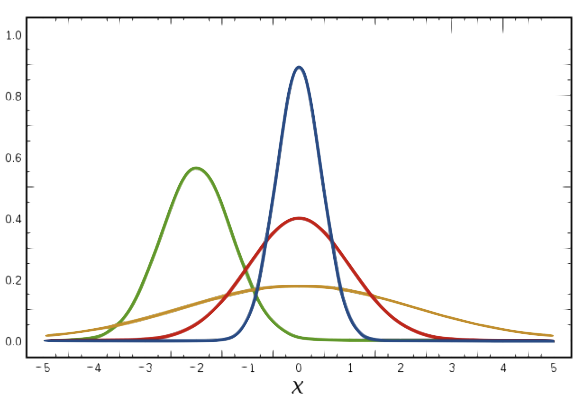
\includegraphics[width=.45\textwidth]{rvs.png}
			
			\textbf{Exercise:} For any scalar $\alpha$,  $\E[\alpha X] = \alpha \E[X]$. $\Var[\alpha X] = \alpha^2 \Var[X]$.
		\end{center} 
	\end{frame}
	
	\begin{frame}
		\frametitle{probability review}
		Let $A$ and $B$ be \emph{random events}. 
		\begin{itemize}
			\item \textbf{Joint Probability}: \hspace{1em} $\Pr(A\cap B)$. Probability that both events happen.
			\item \textbf{Conditional Probability}: \hspace{1em}$\Pr(A\mid B) = \frac{\Pr(A\cap B)}{\Pr(B)}$. Probability $A$ happens conditioned on the event that $B$ happens.
			\item \textbf{Independence}: \hspace{1em} $A$ and $B$ are independent events if:
			$\Pr(A\mid B) = \Pr(A)$. 
		\end{itemize}
		Alternative definition of independence:
		\begin{align*}
			\Pr(A\cap B)  = \Pr(A)\cdot \Pr(B).
		\end{align*}
	\end{frame}
	
	\begin{frame}
		\frametitle{probability review}
		\textbf{Example:} What is the probability that for two independent dice rolls taking values uniformly in $\{1,2,3,4,5,6\}$, the first roll comes up odd and the second is $< 3$?
		
		\vspace{3em}
		Let $X$ and $Y$ be \emph{random variables}. $X$ and $Y$ are independent if, for all events $s, t$, the \emph{random events} $[X = s]$ and $[Y = t]$ are independent.
	\end{frame}
	
	\begin{frame}
		\frametitle{the most powerful theorem in all of probability?}
		\textbf{Linearity of expectation:}
		\begin{align*}
			\E[X + Y] = \E[X] + \E[Y]
		\end{align*}
		\vspace{4em}
	\end{frame}
	
	\begin{frame}
		\frametitle{related equations}
		\begin{center}
			\textbf{Always, sometimes, or never?}
		\end{center}
		
		For random variables $X,Y$:
		\begin{itemize}
			\item $\E[XY] = \E[X]\cdot\E[Y]$. 
			\vspace{2em}
			\item $\Var[X + Y] = \Var[X] + \Var[Y]$. 
			\vspace{2em}
			\item $\Var[X] = \E[X^2] - \E[X]^2$.
		\end{itemize}
	\end{frame}
	
	\begin{frame}
		\frametitle{first application}
		You run a web company that is considering contracting with a vendor that provides CAPTCHAs for logins.
		\begin{center}
			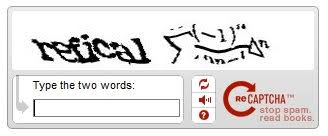
\includegraphics[width=.5\textwidth]{latex_captcha.jpeg}
		\end{center}
		They claim to have a data base of $n = \mathbf{1,000,000}$ unique CAPTCHAs in their database, and a random one will be shown on each API call to their service. They give you access to a test API so you can try it out.
		
		\textbf{Question:} Roughly how many queries to the API, $m$, would you need to independently verify the claim that there are $\sim 1$ million unique puzzles?  
	\end{frame}
	
	\begin{frame}
		\frametitle{first application}
		\textbf{First attempt:} Count how many unique CAPTCHAs you see, until you find $1,000,000$ or close to it. Declare that you are satisfied. 
		
		As a function of $n$, roughly how many API queries $m$ do you need?
	\end{frame}
	
	\begin{frame}
		\frametitle{a different approach}
		\textbf{Clever alternative:} Count how many \emph{duplicate} CAPTCHAs you see.
		
		\vspace{.5em}
		\begin{center}
			
\includegraphics[width=.6\textwidth]{duplicates.png}
			\vspace{.5em}
		\end{center}
	
	 If you see the same CAPTCHA on query $i$ and $j$, that's one duplicate. If you see the same CAPTCHA on queries $i$, $j$, and $k$, that's three duplicates: $(i,j)$, $(i,k)$, $(j,k)$. 
	\end{frame}
	
	\begin{frame}
		\frametitle{formalizing the problem}
		\textbf{Question:} How many duplicates do we expect to see?
		
		Let $D_{i,j} = 1$ if queries $i,j$ return the same CAPTCHA, and $0$ otherwise. 
		
		This is called an \alert{indicator random variable}. $D_{i,j} = \mathbbm{1}[\text{CAPTCHA $i$ equals CAPTCHA $j$}]$.
		
		Number of duplicates $D$ is :
		\begin{align*}
			D = \sum_{\substack{i,j \in \{1,\ldots, m\}\\ i < j}} D_{i,j}.
		\end{align*}
		
		\begin{center}
			\Large What is $\E[D]$?
		\end{center}
	\end{frame}
	\begin{frame}
		\frametitle{formalizing the problem}
		\textbf{Question:} How many duplicates do we expect to see? Formally, what is $\E[D]$?
		\begin{align*}
			\E[D] = \hspace{20em}
		\end{align*}
		
		\vspace{9em}
		\begin{block}{\vspace*{-3ex}}
			\small $n = $ number of CAPTCHAS in database, $m=$ number of test queries. $D_{i,j} =$ indicator for event CAPTCHA $i$ and $j$ collide. 
		\end{block}
	\end{frame}
	
	\begin{frame}
		\frametitle{some hard numbers}
		Suppose you take $m = 1000$ queries and see $10$ duplicates. How does this compare to the expectation if the database actually has $n = 1,000,000$ unique CAPTCHAs?
		\vspace{1em}
		\begin{align*}
			\E[D] = \hspace{13em} 
		\end{align*}

			
		Something seems wrong... this random variable $D$ came up much larger than it's expectation. 
		
		\begin{center}
			\alert{\textbf{Can we say something formally?}}
		\end{center}
		
		\vspace{4em}
		\begin{block}{\vspace*{-3ex}}
			\small $n = $ number of CAPTCHAS in database, $m=$ number of test queries.
		\end{block}
	\end{frame}
	
	\begin{frame}
		\frametitle{concentration inequality}
		One of the most important tools in analyzing randomized algorithms. Tell us how likely it is that a random variable $X$ deviates a certain amount from its expectation $\E[X]$. 
		
		We will learn three fundamental concentration inequalities:
		\begin{enumerate}[label=\arabic*.]
			\item \textbf{\alert{Markov's Inequality}}.
			\begin{itemize}
				\item Applies to \emph{non-negative} random variables.
			\end{itemize}
			\item Chebyshev's Inequality.
			\begin{itemize}
				\item Applies to random variables with \emph{bounded variance}.
			\end{itemize}
			\item Hoeffding/Bernstein/Chernoff bounds.
			\begin{itemize}
				\item Apply to \emph{sums} of \emph{independent random variables}.
			\end{itemize}
		\end{enumerate}
		
	\end{frame}
	
	\begin{frame}
		\frametitle{markov's inequality}
		\textbf{Theorem (Markov's Inequality):} For any random variable $X$ which only takes \emph{non-negative} values, and any positive $t$, 
		\begin{align*}
			\Pr[X \geq t] \leq \frac{\E[X]}{t}.
		\end{align*}
		Equivalently,
		\begin{align*}
			\Pr[X \geq \alpha \cdot\E[X]] \leq \frac{1}{\alpha}.
		\end{align*}
		
		\textbf{Proof:}
		\vspace{9em}
	\end{frame}
	
	\begin{frame}
		\frametitle{application to captcha problem}
		Suppose you take $m = 1000$ queries and see $10$ duplicates. How does this compare to the expectation if the database actually has $n = 1,000,000$ unique CAPTCHAs?
		\begin{align*}
			\E[D] = \frac{m(m-1)}{2n} = .4995.
		\end{align*}
		
		\textbf{By Markov's}:
		\begin{align*}
			\Pr[D \geq 10] \leq \frac{\E[D]}{10} < .05 \text{ if $n$ actually equals $1$ million}. 
		\end{align*}
		
		We can be pretty sure we're being scammed...
		
		\vspace{1em}
		\begin{block}{\vspace*{-3ex}}
			\small $n = $ number of CAPTCHAS in database, $m=$ number of test queries.
		\end{block}
	\end{frame}
	
	\begin{frame}
		\frametitle{general bound}
		\textbf{Alternative view:} If $\E[D] = \frac{m(m-1)}{2n}$, then a natural estimator for $n$ is:
		\begin{align*}
			\tilde{n} = \frac{m(m-1)}{2D}.
		\end{align*}
		With a little more work it is possible to show the following: 
		
		\textbf{Claim:} If $m = \Omega\left(\frac{\sqrt{n}}{\epsilon}\right)$, then with probability $9/10$, $(1-\epsilon)n \leq \tilde n \leq (1+\epsilon) n$. This is a two-sided \alert{multiplicative} error guarantee.
		
		\begin{center}
			\textbf{\alert{This is a lot better than our original method that required $O(n)$ queries!}}
		\end{center}
		
		\vspace{6em}
		\begin{block}{\vspace*{-3ex}}
			\small $n = $ number of CAPTCHAS in database, $m=$ number of test queries.
		\end{block}
	\end{frame}
	
	\begin{frame}
		\frametitle{mark and recaptcha}
		\textbf{Fun facts}:
		\begin{itemize}
			\item Known as the ``mark-and-recapture'' method in ecology.
			\item Can also be used by webcrawlers to estimate the size of the internet, a social network, etc. 
		\end{itemize}
		\begin{figure}
			\begin{subfigure}[t]{0.4\textwidth}
				\centering
				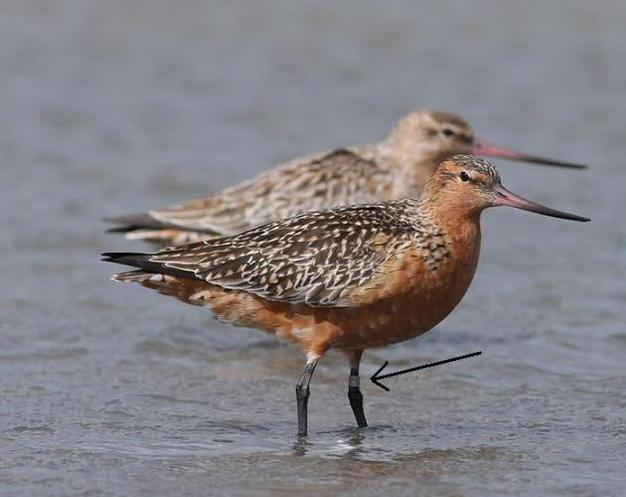
\includegraphics[width=\textwidth]{bird.jpg}
			\end{subfigure}
			\hfill
			\begin{subfigure}[t]{0.4\textwidth}
				\centering
				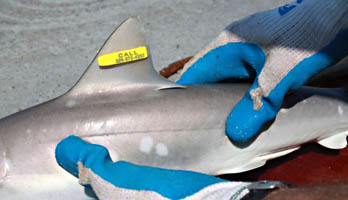
\includegraphics[width=\textwidth]{fish.jpg}
			\end{subfigure}
		\end{figure}
		This is also closely related to the \emph{birthday paradox.}
	\end{frame}
	
	\begin{frame}
		\frametitle{first set of tools}
		\begin{center}
			\textbf{\large\alert{Linearity of Expectation + Markov's Inequality}}\vspace{.5em}
			
			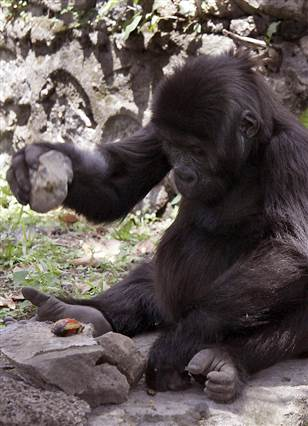
\includegraphics[width=.3\textwidth]{monkey_using_tools.jpg}
			
			Primitive but powerful toolkit, which can be applied to a wide variety of applications!
		\end{center}	
	\end{frame}
	
	\begin{frame}
		\frametitle{the frequent items problem}
		\small
		\textbf{$k$-Frequent Items (Heavy-Hitters) Problem}: Consider a stream of $n$ items $x_1,\ldots, x_n$ with duplicates. Assume there are $u\leq n$ unique items in the stream. Return any item at appears at least $\frac{n}{k}$ times.
		\begin{align*}
			&x_1,\,\, x_2,\,\,x_3,\,x_4,x_5,\,\,x_6,\ldots\hspace{20em}\\
			&v_{10},v_{10},v_2,v_5,v_{10},v_2\ldots\hspace{20em}
		\end{align*}
		
		\begin{itemize}
			\item Finding top/viral items (i.e., products on Amazon, videos watched on Youtube, Google searches, etc.)
			\item Finding very frequent IP addresses sending requests (to detect DoS attacks/network anomalies).
			\item `Iceberg queries' for all items in a database with frequency above some threshold.
		\end{itemize}
		Want very fast detection, without having to scan through database/logs. I.e., want to maintain a running list of frequent items that appear in a stream of data items.
	\end{frame}
	
	\begin{frame}
		\frametitle{the frequent items problem}
		\small
		\textbf{$k$-Frequent Items (Heavy-Hitters) Problem}: Consider a stream of $n$ items $x_1,\ldots, x_n$ with duplicates. Assume there are $u\leq n$ unique items in the stream. Return any item that appears at least $\frac{n}{k}$ times.
		\begin{center}
			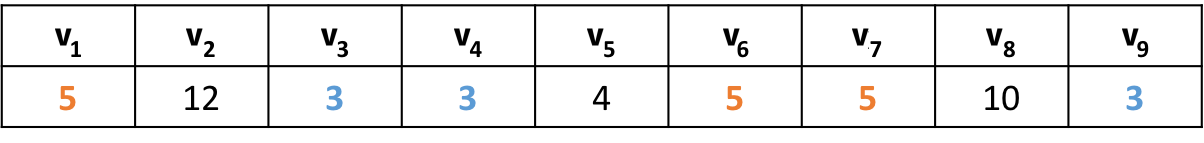
\includegraphics[width=.95\textwidth]{fi.png}
		\end{center}
		\vspace{-.5em}
		\begin{itemize}
			\vspace{.5em}
			\item Trivial with $O(u)$ space -- store the count for each item and return the one that appears $\ge n/k$ times.
			%		\item Can we do it with less space? I.e., without storing counts for all items?
			%		\item \alert{\textbf{What is the maximum number of items that must be returned?}}
			%		\begin{center}
				%			a) \hspace{.5em} $u$ \hspace{1em} b) \hspace{.5em}$k$ \hspace{1em}  c) \hspace{.5em} $n/k$ \hspace{1em}  d) \hspace{.5em} $u/k$
				%		\end{center}
		\end{itemize}
		
	\end{frame}
	
	
	\begin{frame}
		\frametitle{frequent subset mining}
		\small
		\textbf{Example where linear dependence on $u$ is too large:} Find common subsets within a collection of sets. Each subset is an ``item''.
		\begin{center}
			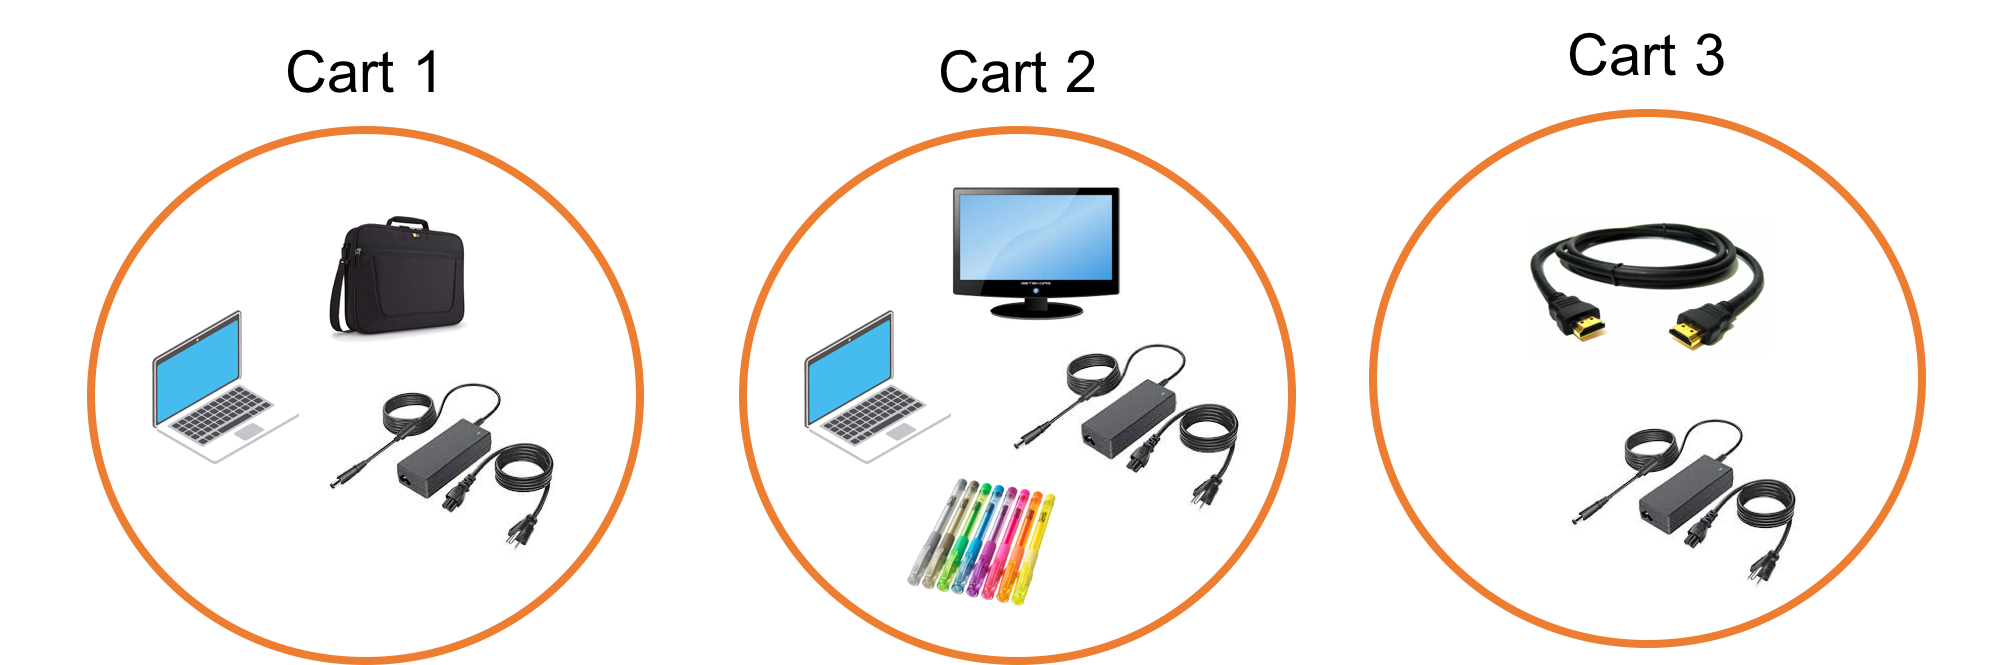
\includegraphics[width=.75\textwidth]{itemset1.png}
		\end{center}
		\begin{itemize}
			\item For product recommendations, the number of pairs of products might grow quadratically with the number of products. Amazon has $12$ million products. $(12 \text{ million})\times 4 \text{ bytes }= 48 \text{ megabytes }$.  $(12 \text{ million})^2\times 4 \text{ bytes }= 576 \text{ terabytes}$ to maintain counts.
			\item For social media recommendations, we might have a set of followers for each Twitter user and want to count frequent subsets of who they follow. Even higher complexity. 
		\end{itemize}
	\end{frame}
	
	\begin{frame}
		\frametitle{approximate frequent elements}
		\textbf{Issue:} Can prove that no algorithm using $o(u)$ space can output just the items with frequency $\ge n/k$. We will only be able to solve the problem \emph{approximately}.
		
		\vspace{1em}
		\textbf{$(\epsilon,k)$-Frequent Items Problem}: Consider a stream of $n$ items $x_1,\ldots, x_n$. Return a set  of items $F$, including \alert{all items that appear $ \geq \frac{n}{k}$ times} and \alert{only items that appear $\geq (1-\epsilon) \cdot \frac{n}{k}$ times}.
		\begin{itemize}
			\item For items with frequencies in $[(1-\epsilon) \frac{n}{k},\frac{n}{k}]$, no output guarantee.
		\end{itemize}
	
%	\begin{center}\textbf{What is the maximum number of items we will return?}\end{center}
	\end{frame}
	
	\begin{frame}
		\frametitle{frequent elements with count-min sketch}
		
		\textbf{Today:} Count-Min Sketch -- a \emph{random hashing} based method for the frequent elements problem.
		
		\begin{center}
			Due to a 2005 paper by Graham Cormode and Muthu Muthukrishnan.
		\end{center}
	
	Solves the slightly different \textbf{point query} problem. Given \emph{any} value $v$, let $f(v) = \sum_{i=1}^n \mathbbm{1}[x_i = v]$ be the number of times $v$ appears in the stream. 
	
	\textbf{Goal:} Return estimate $\tilde{f}(v)$ such that $f(v) \leq \tilde{f}(v) \leq f(v) + \frac{\epsilon}{k}n$ with high probability.
	
	
\textbf{Solving Frequent items:} Just return all items for which $\tilde{f}(v) \geq \frac{n}{k}$.
	\end{frame}
	
	\begin{frame}
		\frametitle{random hash function}
		Let $h$ be a \emph{random function} from $|\mathcal{U}| \rightarrow \{1,\ldots, m\}$. This means that $h$ is constructed by an algorithm using a seed of random numbers, but then the function is fixed. Given input $x\in \mathcal{U}$, it always returns the same output, $h(x)$. 
		
		\textbf{Definition: Uniformly Random Hash Function.} 
		A random function $h: \mathcal{U}\rightarrow \{1, \ldots, m\}$ is called uniformly random if:
		\begin{itemize}
			\item $\Pr[h(x) = i] = \frac{1}{m}$ for all $x\in \mathcal{U}$, $i\in \{1,\ldots, m\}$.  
			\vspace{.5em}
			\item $h(x)$ and $h(y)$ are independent r.v.'s for all $x,y\in \mathcal{U}$. 
			\begin{itemize}
				\vspace{.5em}
				\item Which implies that $\Pr[h(x) = h(y)] = $ 
			\end{itemize}
		\end{itemize}
		
		\vspace{3em}
		\begin{block}{\vspace*{-3ex}}
			\small $\mathcal{U} = $ universe of possible keys, $m=$ number of values hashed to.
		\end{block}
	\end{frame}
	
	\begin{frame}
		\frametitle{random hash function}
		\textbf{Caveat:}
		It is not possible to efficiently implement uniform random hash functions! But:
		\begin{itemize}
			\item In practice ``random looking'' functions like MD5, SHA256, etc. often suffice.
			\item If we have time, we will discuss weaker hash functions (in particular, \emph{universal functions}) which suffice for our application, and are efficient to implement.
		\end{itemize}	
		For now, \textbf{assume} we have access to a uniformly random hash function. This is an assumption we will use in future lectures as well. 
	\end{frame}
	
	
	
	\begin{frame}
		\frametitle{count-min sketch}
		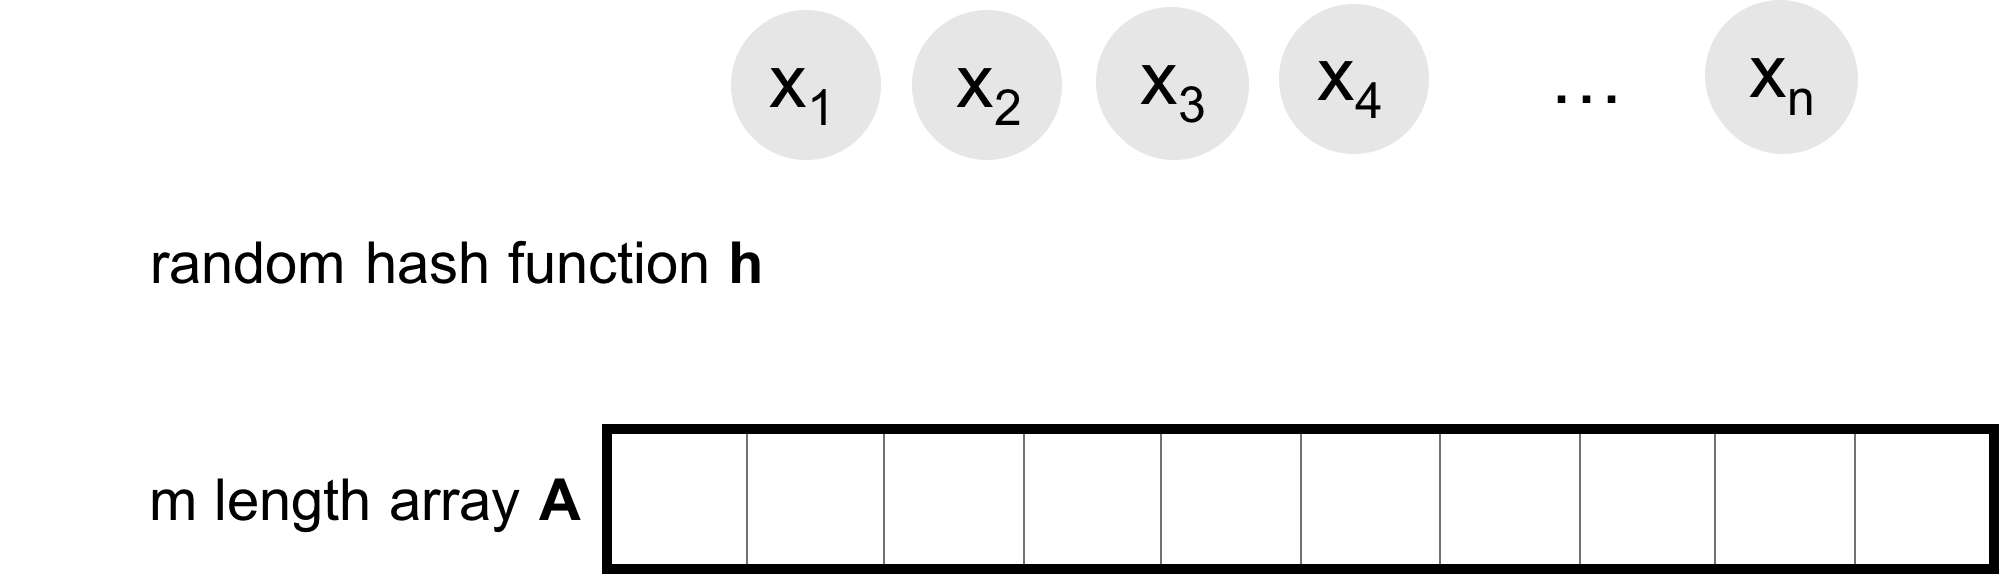
\includegraphics[width=.85\textwidth]{cm0.png}
		
		\textbf{Count-Min Update:}
		\begin{itemize}
			\item Choose random hash function $h$ mapping to $\{1, \ldots, m\}$.
			\item For $i = 1, \ldots, n$
			\begin{itemize}
				\item Given item $x_i$, set $\bv{A}[h(x_i)] = \bv{A}[h(x_i)] + 1$
			\end{itemize}
		\end{itemize}
		
		
		\vspace{3em}
		\begin{block}{\vspace*{-3ex}}
			${h}$: random hash function. $m$: size of Count-Min sketch array.
		\end{block}
	\end{frame}
	
	\begin{frame}
		\frametitle{count-min sketch}
		We want to estimate the  frequency of item $v$, $f(v) = \sum_{i=1}^n \mathbbm{1}[x_i = v]$. To do this using our small space ``sketch'' $\bv{A}$, return  $\tilde{f}(v) = A[\bv{h}(v)]$.
		\vspace{.5em}
		
		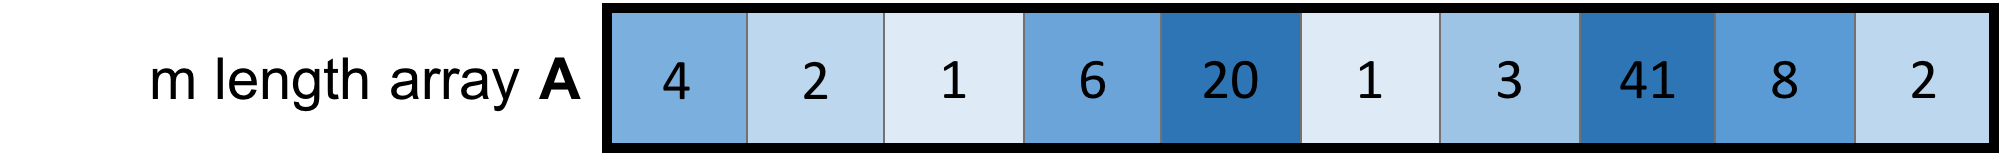
\includegraphics[width=.85\textwidth]{cm5.png}
		
		\textbf{Claim 1:} We always have $\bv{A}[\bv{h}(v)] \ge f(v)$. \alert{Why?}
		
		\vspace{7em}
		\begin{block}{\vspace*{-3ex}}
			\small $f(v)$: frequency of $v$ in the stream. ${h}$: random hash function. $m$: size of Count-Min sketch array.
		\end{block}
	\end{frame}
	
	\begin{frame}
		\frametitle{count-min sketch accuracy}
		\begin{align*}
			\bv{A}[\bv{h}(v)] = f(v) + \underbrace{\sum_{y  \neq v} \mathbbm{1}[\bv h(y) = \bv{h}(v)]\cdot f(y)}_{\text{error in frequency estimate}}
		\end{align*}
		
		\vspace{-2em}
		\small
		\textbf{Expected Error:} 
		\begin{align*}
			\E \left [ \sum_{y  \neq v } \mathbbm{1}[\bv h(y) = \bv{h}(v)]\cdot f(y) \right ] = \hspace{20em}
		\end{align*}
		
	\end{frame}
	
	\begin{frame}
		\frametitle{count-min sketch accuracy}
		\begin{align*}
			\bv{A}[\bv{h}(v)] = f(v) + \underbrace{\sum_{y  \neq v} \mathbbm{1}[\bv h(y) = \bv{h}(v)]\cdot f(y)}_{\text{error in frequency estimate}}
		\end{align*}
		
		\textbf{Expected Error:} 
		\begin{align*}
			\E \left [ \sum_{y  \neq v} \mathbbm{1}[\bv h(y) = \bv{h}(v)]\cdot f(y) \right ] \leq \frac{n}{m}
		\end{align*}
		
		\alert{What is a bound on probability that the error is $\ge \frac{2n}{m}$?}
		
		\smallskip
		\textbf{Markov's inequality:} $\Pr \left [  \sum_{y  \neq x: \bv h(y) = \bv{h}(x)} f(y) \ge \frac{2n}{m}\right ] \le $
		
		\begin{block}{\vspace*{-3ex}}
			\small $f(v)$: frequency of $v$ in the stream. ${h}$: random hash function. $m$: size of Count-Min sketch array.
		\end{block}
	\end{frame}
	
	
	\begin{frame}
		\frametitle{count-min sketch accuracy}
		\begin{center}
			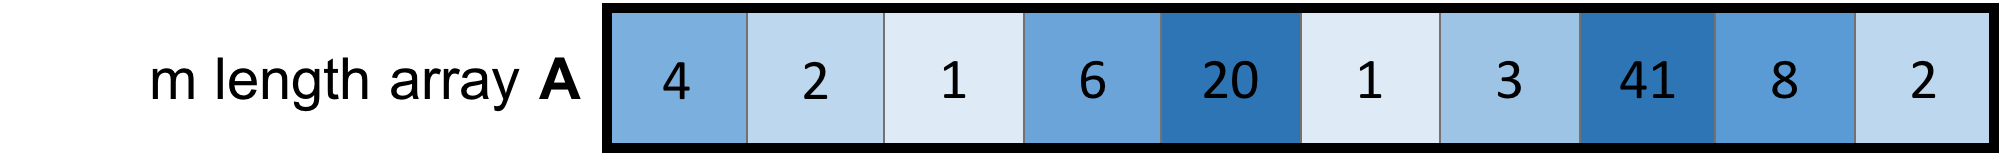
\includegraphics[width=\textwidth]{cm5.png}
		\end{center}
		\textbf{Claim:} For any $v$, with probability at least $1/2$, 
		$$f(v) \le 	\bv{A}[\bv{h}(v)] \le f(v) + \frac{2n}{m}.$$
		
		To solve the point query problem with error $\frac{\epsilon}{k}n$, 
		set $m = \hspace{2em}$
		
		\vspace{3em}
		\alert{\textbf{How can we improve the success probability?}}

		\vspace{1em}
		\begin{block}{\vspace*{-3ex}}
			\small $f(v)$: frequency of $v$ in the stream. ${h}$: random hash function. $m$: size of Count-Min sketch array.
		\end{block}
	\end{frame}
	
	\begin{frame}
		\frametitle{count-min sketch accuracy}
		\begin{center}
			\hspace{-2em}
			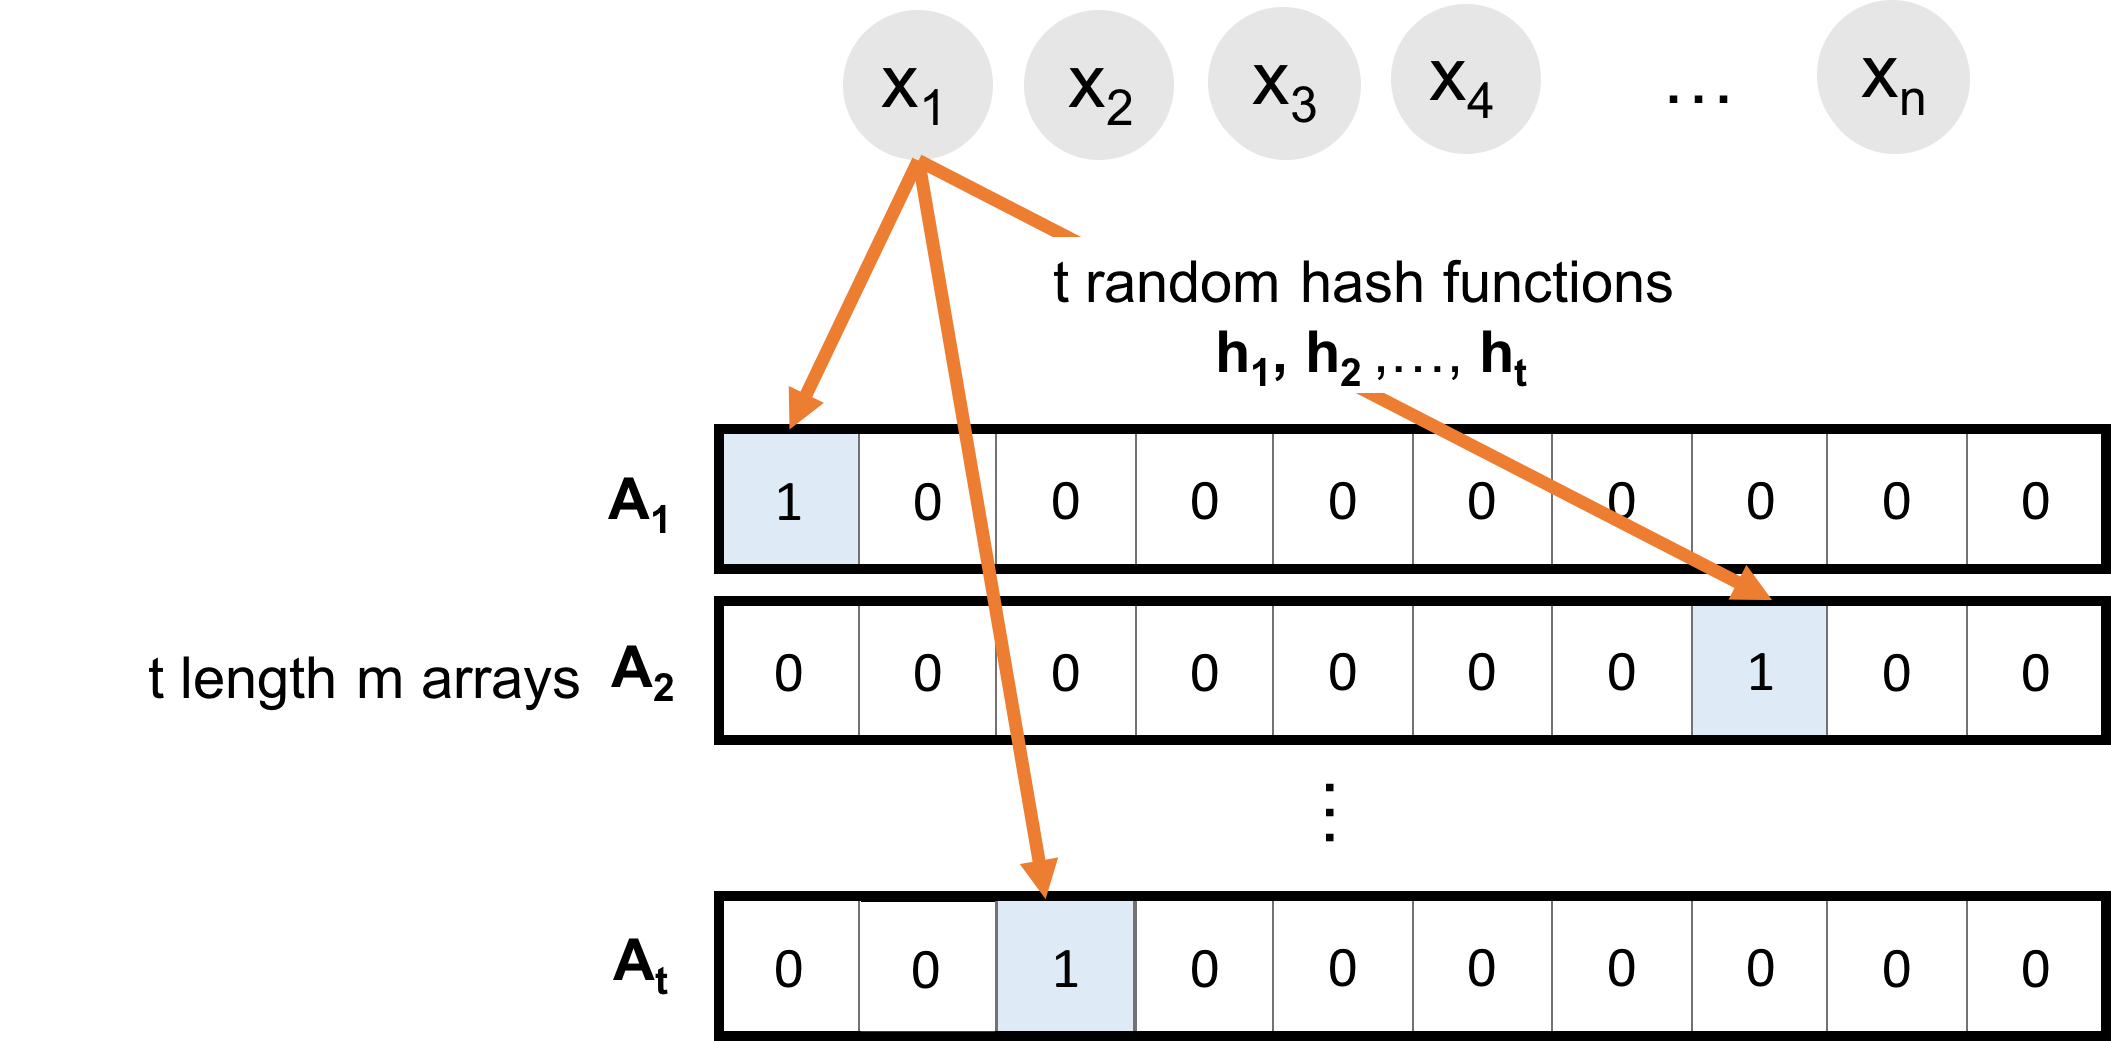
\includegraphics[width=.85\textwidth]{cmm1.png}
		\end{center}
		
		\vspace{4em}
		\begin{block}{\vspace*{-3ex}}
			\small $f(v)$: frequency of $v$ in the stream. $h_1, \ldots, h_t$: multiple random hash functions. $m$: size of $t$ Count-Min sketch arrays.
		\end{block}
	\end{frame}
	
	\begin{frame}
		\frametitle{count-min sketch accuracy}
		\begin{center}
			\hspace{-2em}
			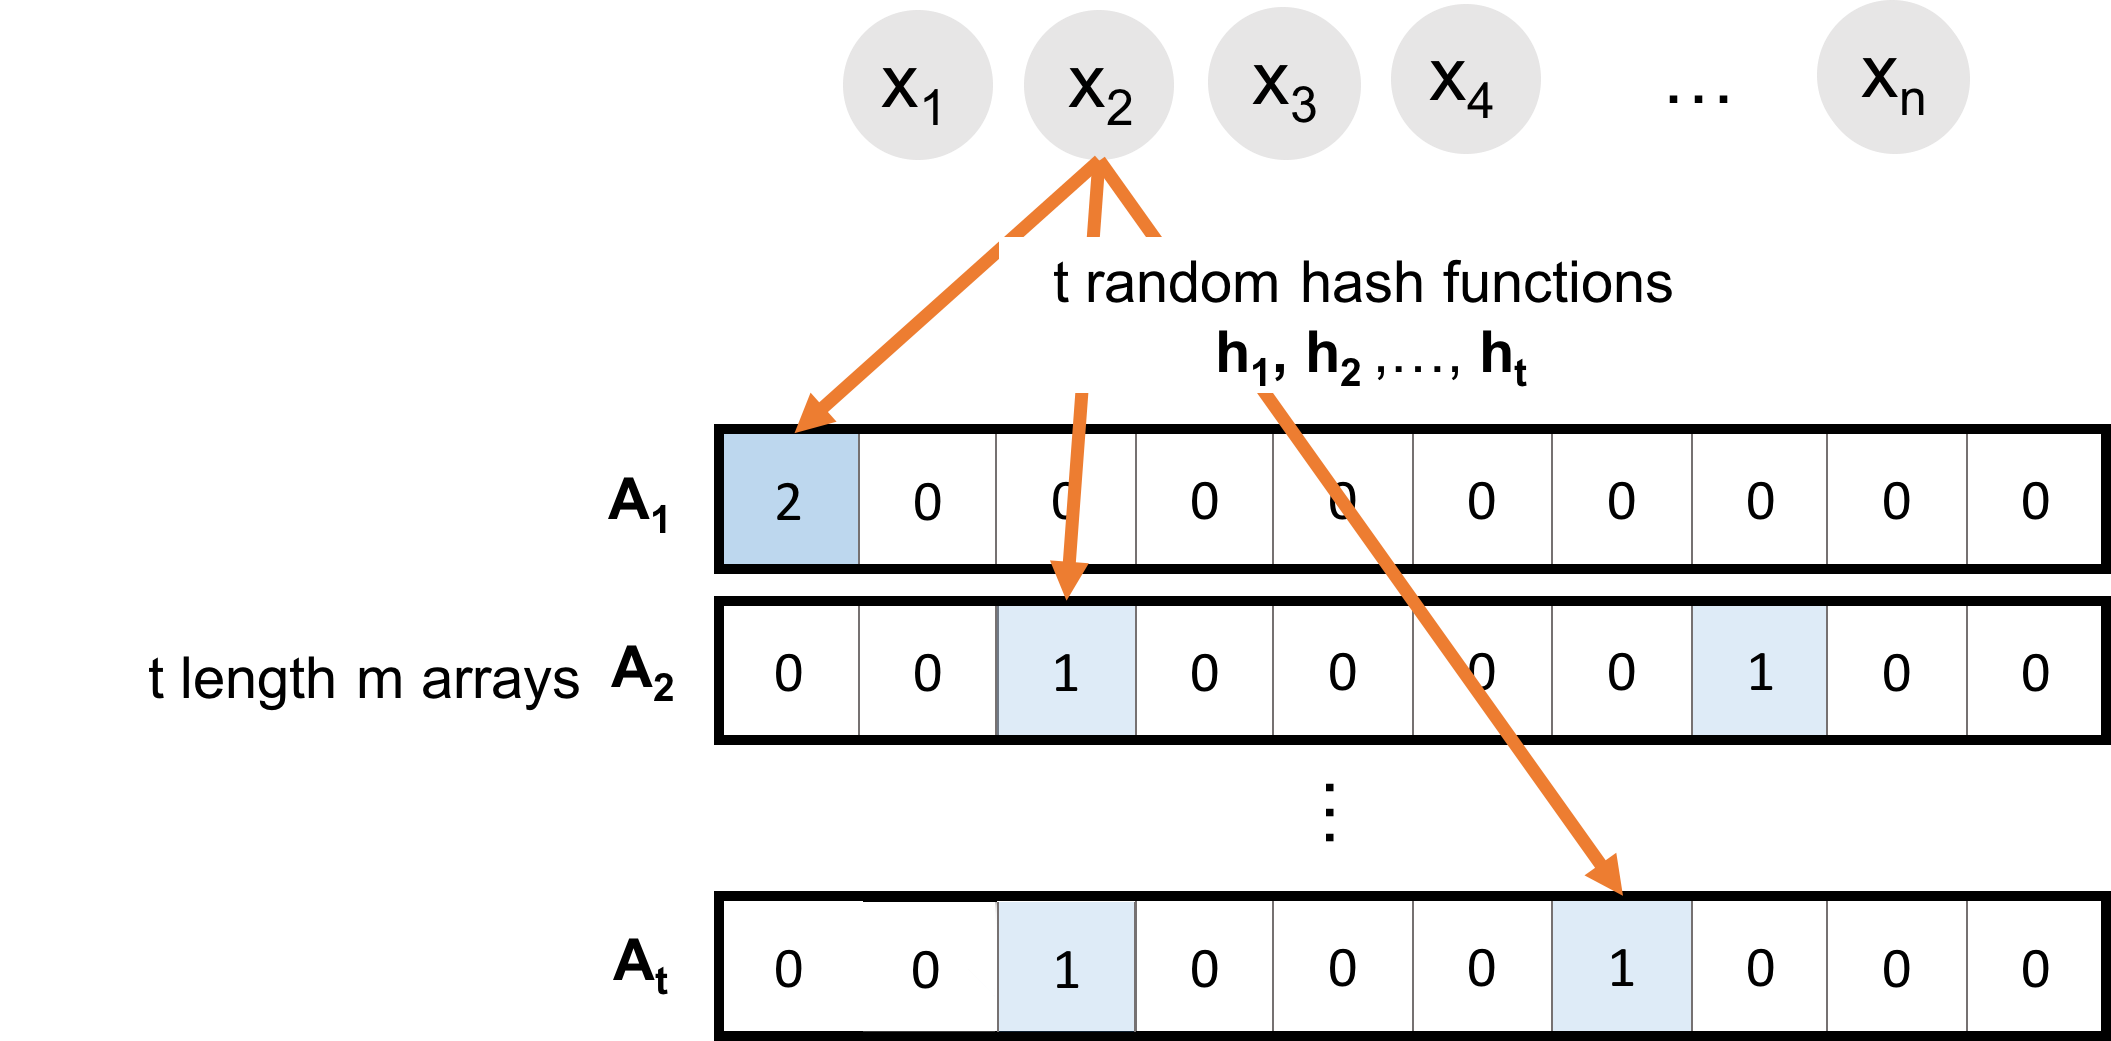
\includegraphics[width=.85\textwidth]{cmm2.png}
		\end{center}
		
		\vspace{4em}
		\begin{block}{\vspace*{-3ex}}
			\small $f(v)$: frequency of $v$ in the stream. $h_1, \ldots, h_t$: multiple random hash functions. $m$: size of $t$ Count-Min sketch arrays.
		\end{block}
	\end{frame}
	
	\begin{frame}
		\frametitle{count-min sketch accuracy}
		\begin{center}
			\hspace{-2em}
			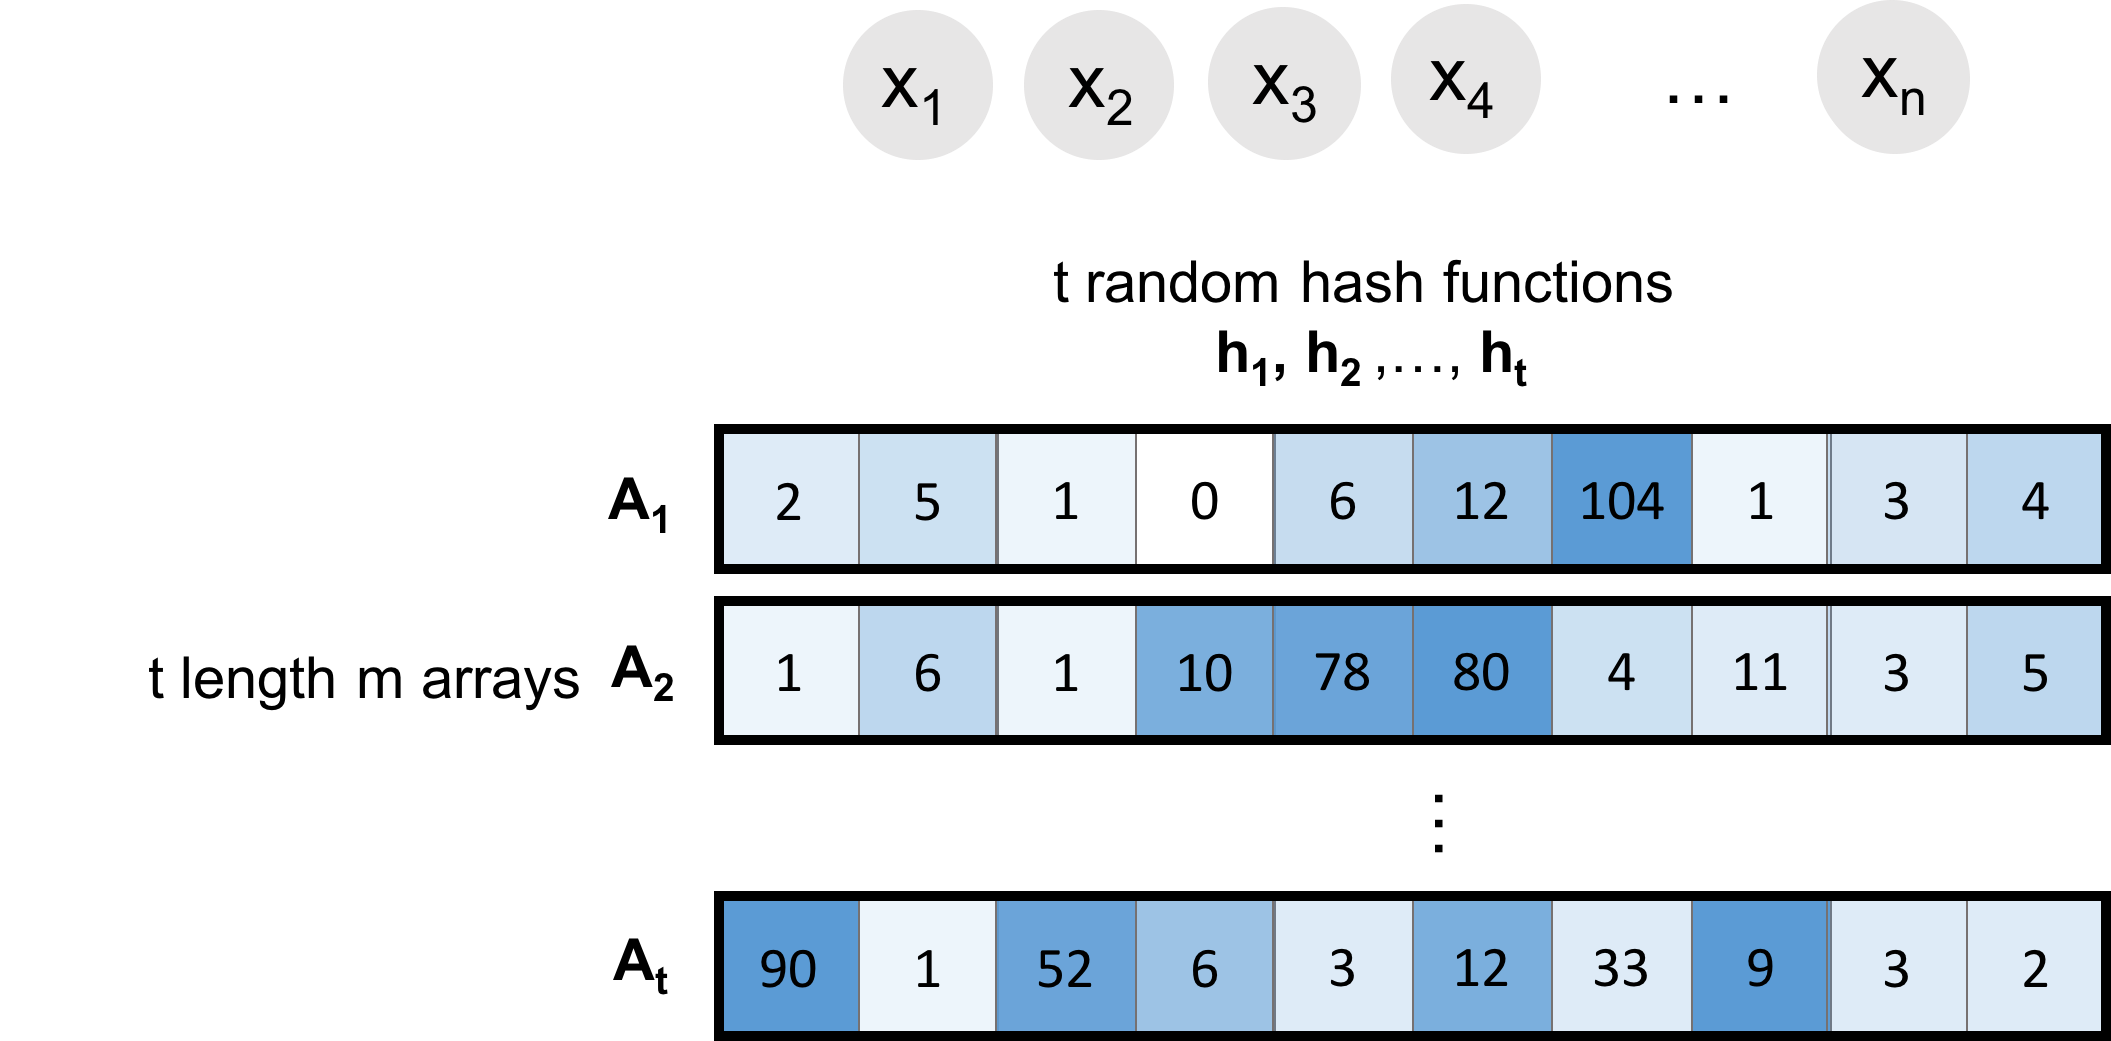
\includegraphics[width=.85\textwidth]{cmm4.png}
		\end{center}
		
		\vspace{4em}
		\begin{block}{\vspace*{-3ex}}
			\small $f(v)$: frequency of $v$ in the stream. $h_1, \ldots, h_t$: multiple random hash functions. $m$: size of $t$ Count-Min sketch arrays.
		\end{block}
	\end{frame}
	
	\begin{frame}
		\frametitle{count-min sketch accuracy}
		\begin{center}
			\hspace{-2em}
			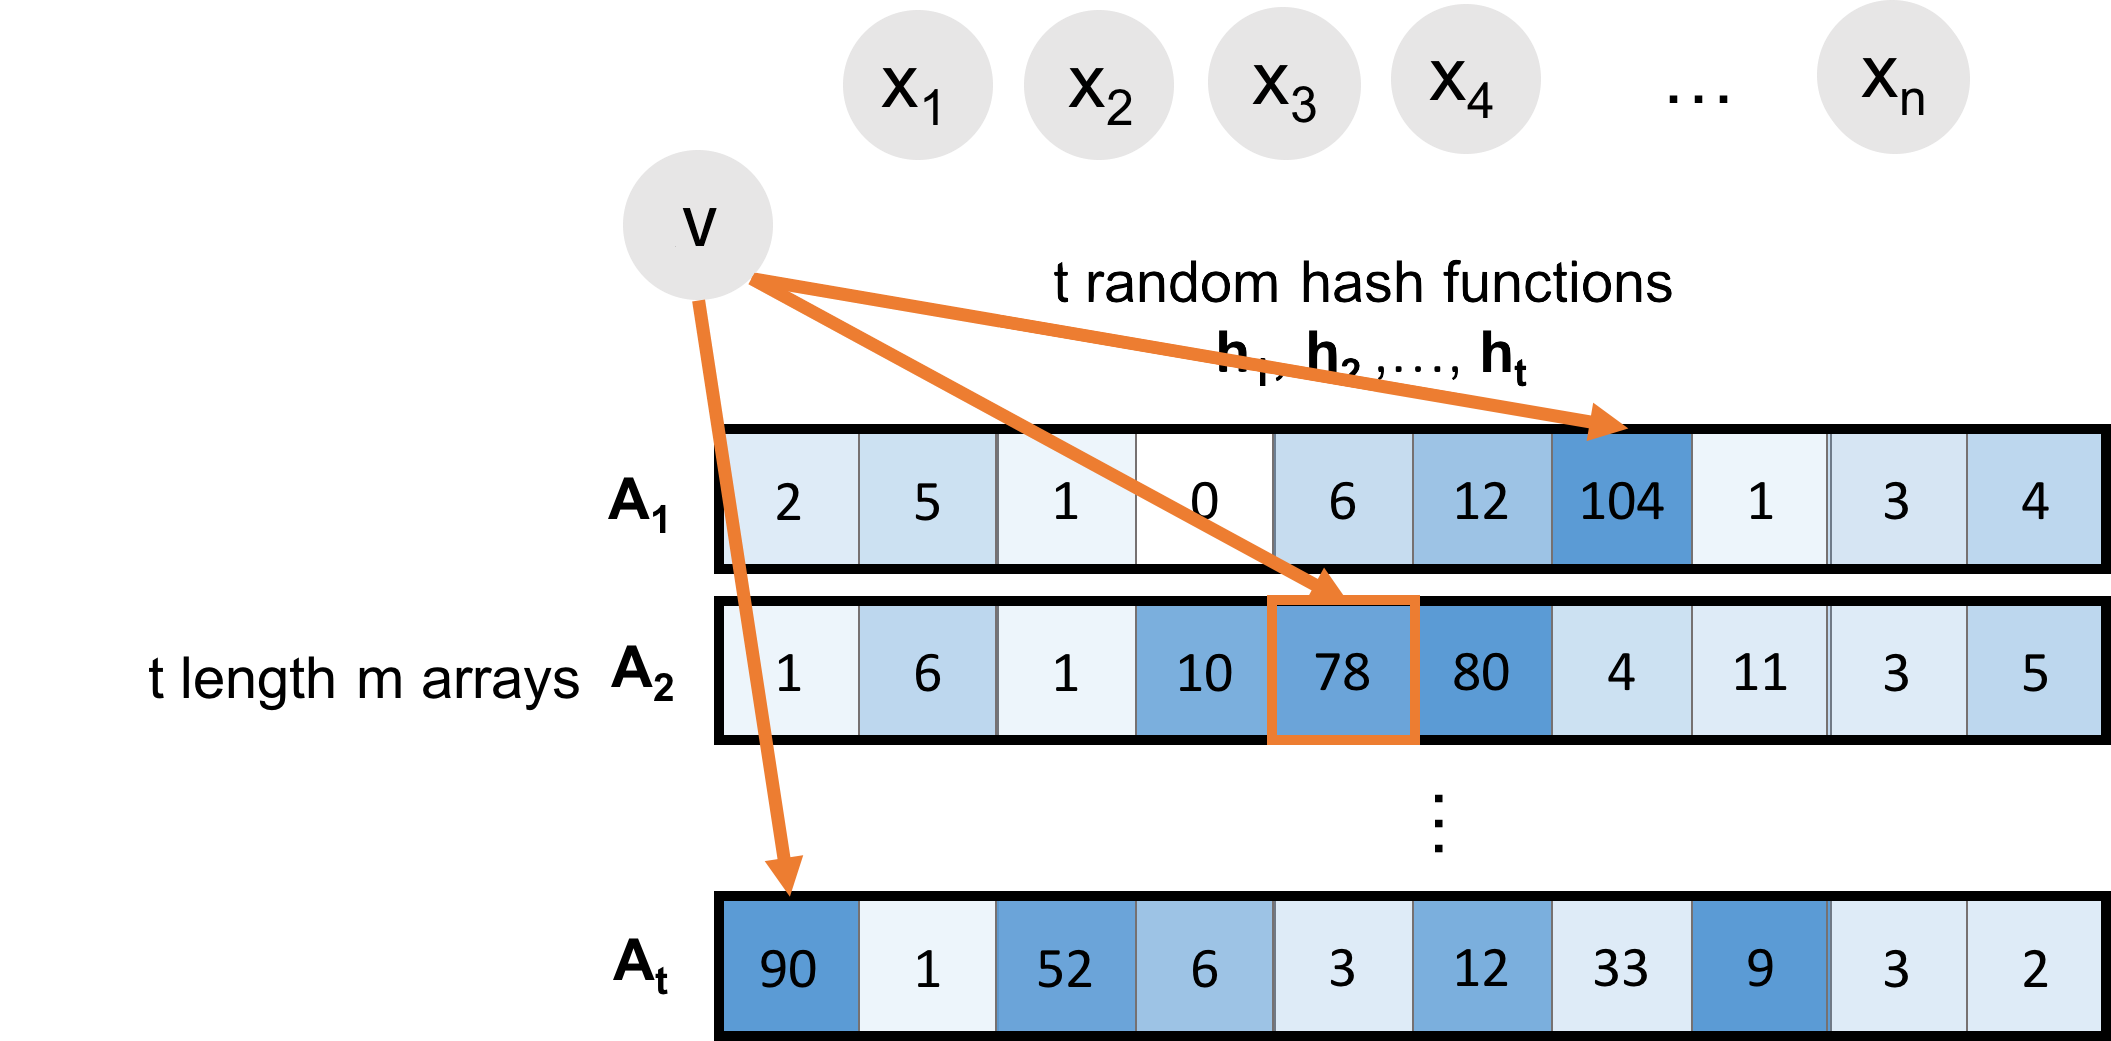
\includegraphics[width=.85\textwidth]{cmm5.png}
		\end{center}
		Estimate $f(v)$ with $\tilde{f}(v) = \min_{i \in [t]} \bv{A}_i[\bv{h}_i(v)]$. (Count-\alert{\textbf{Min}} sketch)
		\begin{center}
			Why min instead of mean or median?
		\end{center}
	\end{frame}
	
	
	\begin{frame}
		\frametitle{count-min sketch accuracy}
		\small
		\begin{center}
			\hspace{-2em}
			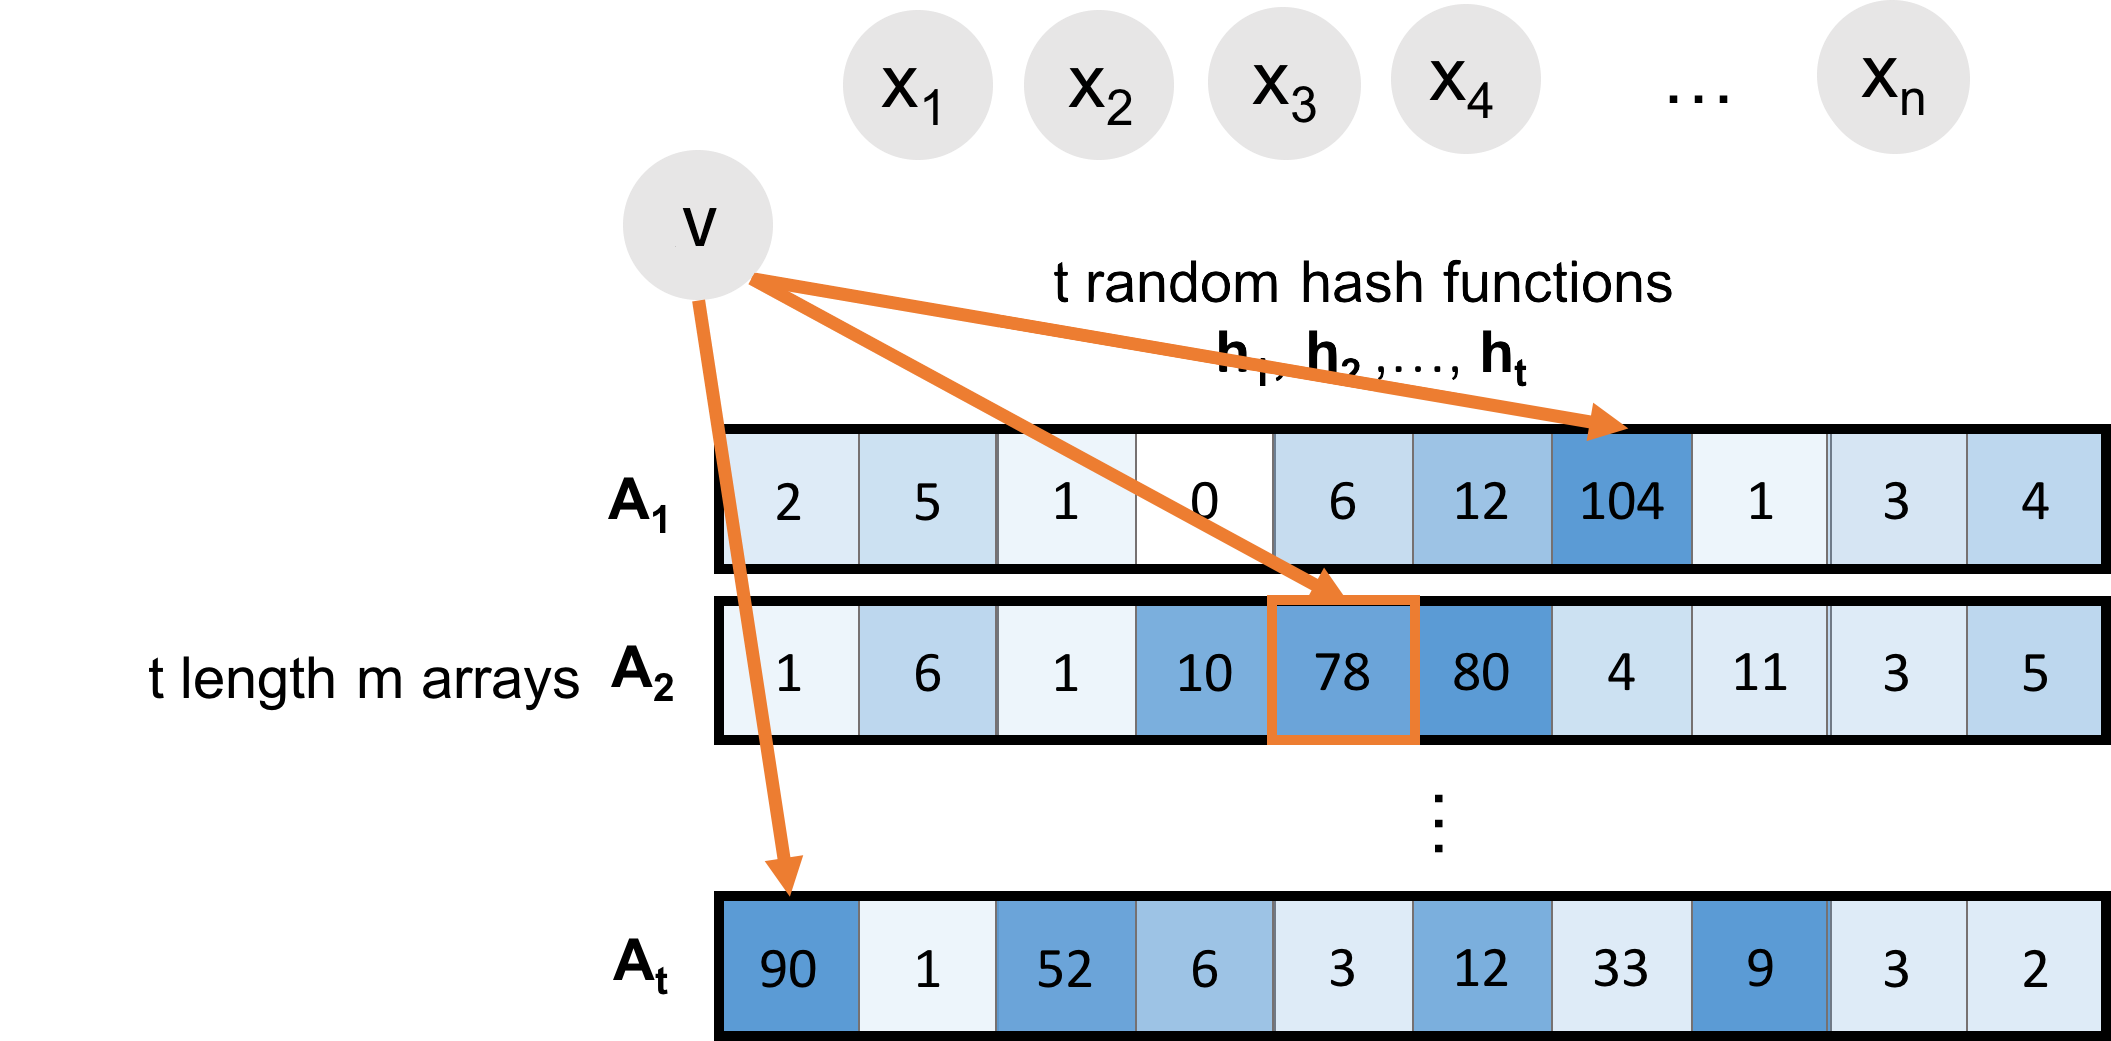
\includegraphics[width=.65\textwidth]{cmm5.png}
		\end{center}
		Estimate $f(v)$ with $\tilde{f}(v) = \min_{i \in [t]} \bv{A}_i[\bv{h}_i(v)]$.
		\begin{itemize}
			\item For every $v$ and $i$ and $m = \frac{2k}{\epsilon}$, we know that with prob. $\ge 1/2$:
			\vspace{-.5em}
			$$f(v) \le \bv{A}_i[\bv{h}_i(v)] \le f(v) + \frac{\epsilon n}{k}.$$
			\item \alert{\textbf{$\Pr [f(v) \le \tilde{f}(v) \le f(v) + \frac{\epsilon n}{k}] \geq$}}
			\item To get a good estimate with probability $\ge 1-\delta$, 
			$$\textbf{set } t = \hspace{3em}$$.
		\end{itemize}
	\end{frame}
	
	\begin{frame}
		\frametitle{count-min sketch}
		\textbf{Upshot:} Count-Min sketch lets us estimate the frequency of each item in a stream up to error $\frac{\epsilon}{k}n$ with probability $\ge 1-\delta$ in $O \left  (\log(1/\delta) \cdot \frac{k}{\epsilon} \right )$ space.
	
	\vspace{4em}
	\textbf{Caveat:} This is a \emph{for each} $v$ guarantee. We actually want a \emph{for all} $v$ guarantee: i.e. the bound should hold simultaneously for all $v$.
	\end{frame}

\begin{frame}
	\frametitle{use a union bound}
	\begin{lemma}[Union Bound]
		For \emph{any} random events $A_1, \ldots, A_k$:
		\begin{align*}
			\Pr[A_1 \cup A_2 \cup \ldots \cup A_k] \leq \Pr[A_1] + \Pr[A_2] + \ldots +\Pr[A_k].
		\end{align*}
	Here $Pr[A_1 \cup A_2 \cup \ldots \cup A_k]$ means $Pr[A_1 \text{ ``or'' } A_2 \ldots \text{ ``or'' }  A_k]$
	\end{lemma}
	\begin{center}
		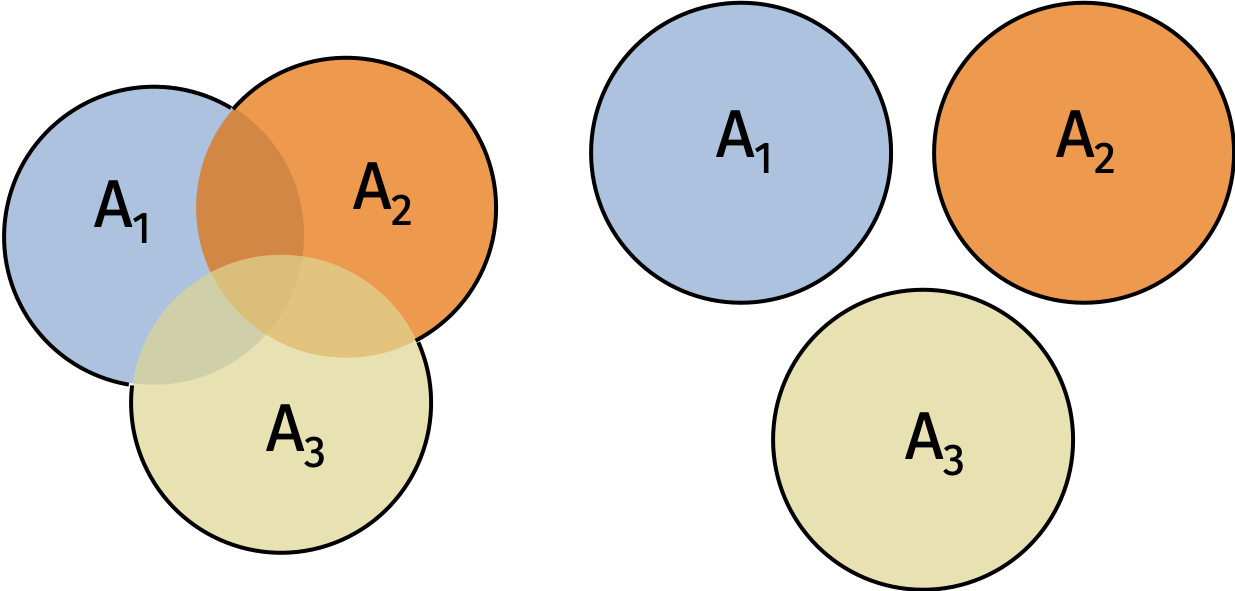
\includegraphics[width=.8\textwidth]{union_bound_proof.png}
		
		\textbf{Proof by picture.}
	\end{center}
\end{frame}

\begin{frame}
	\frametitle{use a union bound}
	The algorithm fails if $|f(v) - \tilde{f}(v)| > \frac{\epsilon}{k} n$ for any $v \in \{v_1, \ldots, v_n\}$. By union bound:
	\begin{align*}
		\Pr[(\text{fail for } v_1) \text{ or } (\text{fail for } v_2)  \text{ or}  \ldots  \text{ or}  (\text{fail for } v_n)] = 
	\end{align*}
	
\end{frame}

\begin{frame}
		\frametitle{final result}
		Set $\delta = \frac{1}{10n}$. With probability $9/10$, Count-Min sketch lets us estimate the frequency of \emph{all} items in a stream up to error $\frac{\epsilon}{k}n$.
		\begin{itemize}
			\item Accurate enough to solve the $(\epsilon,k)$-Frequent elements problem -- just return all $v$ with estimated frequency $\geq n/k$.
		\end{itemize}
\end{frame}

	
	\begin{frame}
		\frametitle{identifying frequent items}
		How do we identify the frequent items without having to look up the estimated frequency for all elements in the stream? 
		
		\textbf{One approach:} 
		\begin{itemize}
			\item When a new item comes in at step $i$, check if its estimated frequency is $\ge i/k$ and store it if so.
			\item At step $i$ remove any stored items whose estimated frequency drops below $i/k$. 
			\item Store at most $O(k)$ items at once and have all items with estimated frequency $\ge n/k$ stored at the end of the stream.
		\end{itemize}
		
	\end{frame}
	
	\begin{frame}
		\frametitle{note on random hash functions}
		Can we weaken our assumption that $h$ is uniformly random?
		\begin{definition}[Universal hash function]
			A random hash function $h: \mathcal{U} \rightarrow \{1, \ldots, m\}$ is \emph{universal} if, for any fixed $x,y\in \mathcal{U}$,
			\begin{align*}
				\Pr[h(x) = h(y)] \leq \frac{1}{m}.
			\end{align*}
		\end{definition}
		\textbf{Claim:} A uniformly random hash-function is universal. 
		
		\textbf{Efficient alternative:} Let $p$ be a prime number between $|\mathcal{U}|$ and $2|\mathcal{U}|$. Let $a,b$ be random numbers in $0,\ldots, p$, $a\neq 0$.
		\begin{align*}
			h(x) = \left[a\cdot x + b \pmod{p}\right] \pmod{m}
		\end{align*} 
		is universal. Lecture notes with proof posted on website. 
	\end{frame}
	
	\begin{frame}
		\frametitle{note on random hash functions}
		Another definition you might come across:
		\begin{definition}[Pairwise independent hash function]
			A random hash function $h: \mathcal{U} \rightarrow \{1, \ldots, m\}$ is pairwise independent if, for any fixed $x,y\in \mathcal{U}, i,j \in \{1\ldots, m\}$,
			\begin{align*}
				\Pr[h(x) = i \cap h(y) = j] = \frac{1}{m^2}.
			\end{align*}
		\end{definition}
		We can naturally extended to $k$-wise independence for $k > 2$, which is strictly stronger, and needed for some applications. 
	\end{frame}
	
	%\begin{frame}
	%	\frametitle{distributing work loads}
	%	\textbf{Another application of hashing:}
	%	
	%	Suppose Google answers map search queries using an army of servers $A_1, \ldots, A_q$. Given a query like ``new york to rhode island'', common practice is to choose a random hash function $h \rightarrow \{1\ldots, q\}$ and to route this query to server:
	%	\begin{align*}
		%		A_{h(\text{``new york to rhode island'})}
		%	\end{align*}
	%
	%	\begin{center}
		%		\alert{\textbf{Why use a hash function instead of just sending the query to a uniformly random server?}}
		%	\end{center}
	%\end{frame}
	%
	%\begin{frame}
	%	\frametitle{distributing work loads}
	%	\textbf{Online lecture:} We will see how the Markov bound fails us in analyzing this application of hashing, which will motivate a new tool: the Chebyshev inequality.
	%	
	%\end{frame}
	
	
\end{document} 








